\documentclass{elsart}

\input setbmp
\input seteps
\usepackage{epsfig}
\usepackage{enumerate}
\usepackage{amsmath}
\usepackage{amsthm}
\usepackage{amscd}
\usepackage{amssymb}
\usepackage{rotating}

\usepackage{algorithmic}
\usepackage{algorithm}


\newtheorem{definition}{Definition}[section]
\newtheorem{lemma}{Lemma}[section]
\newtheorem{theorem}{Theorem}[section]
\newtheorem{corollary}{Corollary}[section]

\begin{document}
\bibliographystyle{ieeetr}  

\begin{frontmatter}

\title{Time-series Processing of Large Scale Remote Sensing Data with Extreme Learning Machine over Cloud Infrastructure}

\author[label1]{XXX},
\ead{xxx@zju.edu.cn}
\corauth[cor1]{Corresponding author}
\author[label1,label2]{xxx} and
\author[label1]{xxx}
\address[label1]{Zhejiang University}
\address[label2]{School }

\begin{abstract}
Nowadays, land-cover change detection plays a more and more important role in environment protection and many other fields.
However, the current land-cover change detection methods encounter the problem of low effiency and can't be expanded to parallel computing to deal with fast-growing remote sensing(RS) data.
To solve the above problems, we propose a novel ELM-based land-cover change detection method, in which the supervised classification capability, fast training speed and high generalisation performance of ELM is utilized to efficiently train the land-cover classifier and apply the classifier to time-series satellite imageries' analysis.
As one experiment, we apply our method to the analyis of rapid land use change in Changjiang River Delta over the past two decades due to accelerated urbanization.
Moreover, we prove our method's scability by another experiment of large scale RS imageries processing over the cloud infrastructure.
\end{abstract}

\begin{keyword}
Extreme learning machine, Remote Sensing, Classification, Change Detection, Time-series, MapReduce, Hadoop.
\end{keyword}

\end{frontmatter}

%%%%%%%%%%%%%%%%%%%%%%%%%%%%%%%%%%%%%%%%%%%%%%%%%%%%%%%%%%%
%%%%%%%%%%%%%        Introduction      %%%%%%%%%%%%%%%%%%%%%
%%%%%%%%%%%%%%%%%%%%%%%%%%%%%%%%%%%%%%%%%%%%%%%%%%%%%%%%%%%

\section{Introduction}
Nowdays, the available time-series RS images provide a new way for land-cover change detection which is widely required in various fields.
However, except for the traditional challenge of high accuracy, large scale RS data processing also requires the land-cover change detection to be efficient and highly scalable. 
This paper proposes a novel elm-based land-cover change detection method with faster processing speed and higher scalability, which is practiced on cloud infrastructure. 

\subsection{Land-cover Change Detection with Time-series RS Images}
Change detection is the process of identifying differences in the state of an object or phenomenon by observing it at different times\cite{SINGH1989}.
With the development of satellite technology, massive time-series high resolution multispectral RS images are available for applications.  
By comparing two sets of RS images, taken of the same area at different time, we can manually handle the change detection job by view.
In fact, it is possible for the computer to process the digital RS images, and provide an automatical change detection technology, which is available for large scale processing of RS images.
In summary, time-series RS image-based land-cover change detection method is to identifiy the interesting land-cover changes between "before" time images and "after" time images through RS image digital processing and comparison of RS images in an automatical way.
\par

In the recent decades, timely and accurate change detection of Earth's surface features plays a more and more important role in better decision making.
Automatic change detection can be used in such diverse applications as land usage analysis, disaster monitoring, snow-melt measurements, forest coverage monitoring and other environment changes. 
Especially, land-cover change detection is one of the major direction of change detection application. 
Various papers\cite{Weng2002}\cite{Read2002}\cite{Lunetta2002} have presented their work of applying change detection technology to the analysis of land-use and land-cover. 
Ross S. Lunetta\cite{Lunetta2002} performed the change detection experiment in the biologically complex landscape of the Neuse River Basin, North Carolina using Landsat5 and 7 imagery collected in May of 1993 and 2000. 
Another typcial application is performed by Qihao Weng\cite{Weng2002}, to analysis the rapid land use change taken place in Zhujiang Delta over the past decades with the help of change detection technology.

\subsection{Challenges of Land-cover Change Detection}
In the applications of RS images, land-cover change detection has been a problem for some time.
Among all the factors that cause land-cover change detectoin unavailable to real situations, change detection methods or algorithms used play a key role.
Traditionally, the main challenge to land-cover change detection methods is the detection accuracy.
However, with increase scale of RS images and these images' high resolution, the method's processing speed and scability rise to be another two major challenges. 
\par 
Presently, large data processing has become a hot research topic of computing science. Similarly, in the field of RS data processing, increasing data size also brings some new challenges to processing methods. On one hand, efficient processing method is one of the best solutions to reduce processing time, on the other hand, parallel computing or distributed computing can greatly improve the processing efficency of large scale data. In order to support parallel computing, the scalability of the processing method become another challegne.

\subsection{Major Contributions of Elm-based method}
This paper's major contribution is to propose a novel elm-based method for land-cover change detection. 
Using our method, the analysis of rapid land use change in Changjiang River Delta over the past two decades due to accelerated urbanization is done.
Moreover, the land-cover change detection result is evaluated and compared to the current methods, which use the classifier of BP network and SVM.
The novel approach supports high speed processing of single data set and can be extended to parallel computing on cloud infrastructure for the processing of large scale RS data.
In our experiment, we expand the trained ELM network to hadoop based cloud infrastructure to prove the method's scability.
Through the evaluation of the performance improvement of paralle computing, we prove the method's capability to deal with increasing RS imageries.  
\par
ELM is a recently proposed and widely used machine learning method, with the capability of multiclass classification and universal approximation\cite{Huang2012}\cite{Huang2000}\cite{Zhang2007}\cite{Huang2006}.
One of the major characteristic of ELM is its very fast training processing, which directly increases the processing efficiency of land-cover change detection method.
The other advantage of ELM is the high generalisation performance. Generalisation is the key factor that will decide whether the trained network can be widely applied to large scale RS data.
Moreover, our proposed change detection method also take advantage of ELM's less human intervene for the process of network training.
In conclusion, with ELM's high speed of training, high generalisation and less manual intervene, we design our novel land-cover change detection method to overcome the challenges of large scale RS data processing. 

\section{Related Work}
\subsection{Methods for Land-cover Change Detection}
Land usage analysis and land cover mapping has long been an area of research focus, and a wide range of methods including cross-correlation analysis, post-classification, image differencing, image ratioing, principal components analysis and so on have be explored.
Both the traditional methods post-classification and cross-correlation determine the land-cover change through the "before" time and "after" time classifiction map, and produce comparable result. 
Although both methods are more automatic than the others like image differencing, the unsupervised classifier used result in low accuracy, which is one of the most important challenges that change detection methods face.
The methods of image differencing, image ratioing and principal components analysis involve transformations of the original spectral bands so as to enhance the land cover changes.
These methods and their improvement do increase the accuracy of land-cover change detection, but it is limited to small scale data processing and are lack of automation. 
\par

With the advances of machine learning, several alternativ land-cover change detection methods using neural network are proposed and applied in the analysis of landscape. 
Presently, both supervised and unsupervised neural network algorithms have made progress.
Compared to unsupervised land-cover transitions detection methods, the supervised ones provide more information about the kinds of transitions that occured on the ground and are less affected by the difference atmospheric conditions, sensor calibration, and ground condition\cite{Demir2011}\cite{Clifton2003}
The paper\cite{Clifton2003} presents a technique for using predictive modeling, which predicates "before" and "after" pixel value, to identify unusual changes in imageries.
Begum Demir\cite{Demir2011} present a novel iterative active learning(AL) technique aimed at defining effective multitemporal training sets to be used for the supervised detection of land-cover transitions in a pair of time-series RS imageries.
In comparison, unsupervised approaches require fewer manual intervenes\cite{Patra2006}\cite{Patra2007}\cite{Chen2008}, and are quite suitable in the situations that the ground-truth is always unavailable.
However, the low accuracy of unsupervised classification and predication severely limit the application of unsupervised approaches\par
Although the classification and predication capability of neural network brings much improvement to the traditional land-cover change detection methods, the common and widely applied neural netwokrs, like BP network and SVM, exist several inadequacies.
The most two important aspects that exist room for improvement may be the low speed of training and low generalization.
\subsection{ELM for Remote Sensing Application}
Presently, little work of applying ELM to the field of RS imagery processing has been done. 
Mahesh Pal\cite{Pal2008} did the land cover supervised classification experiment with ELM using remote sensing images.
Wu Jun\cite{Jun2011} revealed the equivalence between ELM and the positive and negative fuzzy rule system. 
Moreover, Wu Jun indicate the claim that ELM can be naturally used for training the positive and negative fuzzy rule system quickly for image classification.
However, only simple comparison of classification cabability between ELM and other classification network was done in both efforts, and no time series images processing work are tried, not along large scale RS iamge processing.


\subsection{ELM Based Methods for Large-scale Data Set Processing}
Extreme learning machine is a new learning algorithm for single-hidden layer feedforward neural networkd(SLFNs) which randomly chooses the input weights and analytically determines the output weights of SLFNs\cite{Huang2004}.
In fact, ELM is to minimize the training error as well as the norm of the output weights\cite{Huang2004}\cite{Huang2006a}, and thus to achieve better generalization performance.
As the hidden nodes, including the input weights and hidden nodes' threshold are randomly generated, $\mathbf{H}$, namely the hidden layer output matrix of the neural network\cite{Huang2003}\cite{Huang1998}, can be directly calcualted, thus greatly reducing the network training time.
\par

As large-scale data set processing has been the trend of present applications, some researchers have paied their attentions to the scapability of ELM methods.
Through improving the scapability, they extend the ELM variant methods to parallel computing infrastructures to deal with large-scale data set training.
Qing He\cite{He2011} proposed to implement an efficient paralled ESVM based on the current and powerful parallel programming framework MapReduce.
Moreover, an incremental learning algorithm for ESVM, which can meet the requirement of online learning to update the existing network, as well as its parallel version, is proposed in \cite{He2011}.
Mark van Heeswijk\cite{Heeswijk2011} compared three distinct ways of accelerating the evaluation of this ensemble of ELMs, and concluded that the GPU-accelerated and parallelized ELM ensemble achieved attractive sppedups over using single CPU.
Yongjiao Sun\cite{Heeswijk2011} propose an OS-ELM based ensemble classification framework for distributed classification in a hierarchical P2P network.
In spite of the above contributions to the scability improvement, their proposed parallel computing methods are limited to the model building process.
Meanwhile, no real applications are applied in and their efficiency on remote sensing imagery processing are known.


\section{ELM-based Method for Land-cover Change Detection}
In this paper, we propose our new land-cover change detection method based on extreme learning machine using time-series RS images.
The change detection is calculated through the comparison between "before" time and "after" time land-cover mapping, which is the result of land-cover classification of RS images.
With the high speed of network training and high generalisation performance of classification, the new method has advantage of fast processing and high scability, compared to the traditional neural network based methods.
Moreover, the new method is extended to cloud infrastructure to deal with large scale RS images processing.

\subsection{Land-cover Change Detection Method}
The whole land-cover change detection method can be divided into two components: training unit and detection unit as shown in Figure 1.
Training unit is to build an ELM networking using preprocessed training and testing samples, which has adjusted hidden node number and can be directly applied to real remote sensing image classification with the highest generalisation performance.
While the detection unit firstly calculates both "before" time land-cover mapping and "after" time land-cover mapping through the classification of time-series remote sensing images using the trained network, and then works out the change detection statistics and change map by means of comparing the pair of time-series land-cover mapping.
\begin{figure}[tbh]
%\centereps{5.0in}{4.0in}{method.eps}
\begin{center}
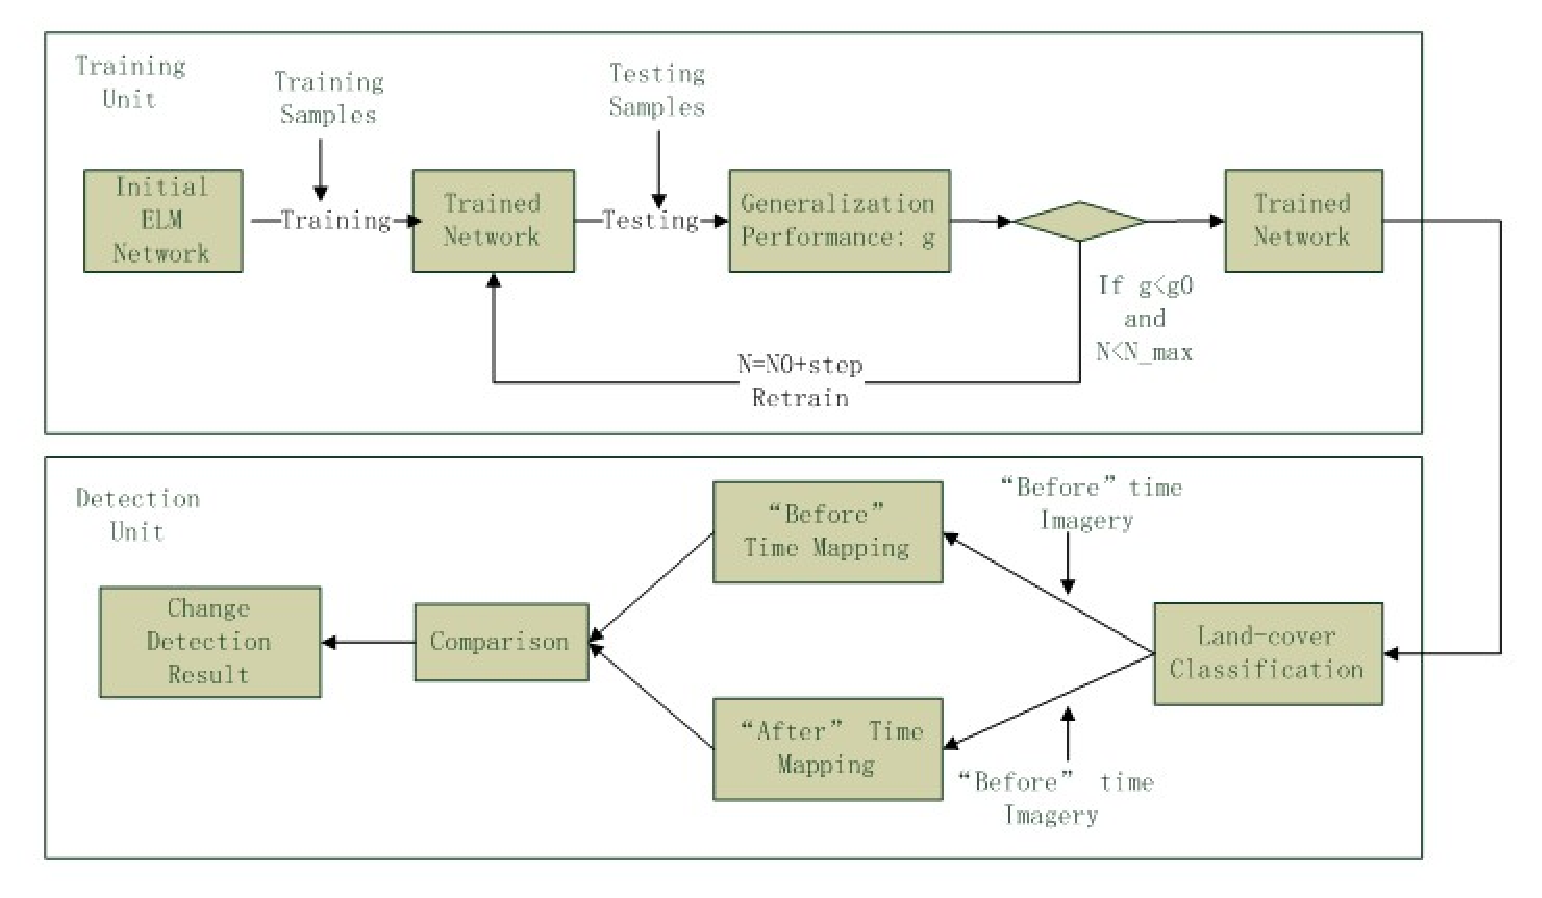
\includegraphics[width=15cm]{method.eps}
\caption{ELM-based Land-cover Change Detection Method}
\label{method}
\end{center}
\end{figure}
\par

\subsubsection{Land-cover Classification and Samples}
According to different terrains area and resolution of remote sensing images, the land-covery can be classified into specific categories. 
In fact, in order to assure the precision, statistical property and representative of the sample, training sample of each category should be selected through visual interpretation and field survey\cite{YuXiu-Lan1999}.
In our application, according to the investigation of land-cover of Taihu Area and the landsat images' resolution, we classify the land-cover into four types as described in Table 1.
\begin{table}[h]
\scriptsize{
\begin{center}
\begin{tabular}[bt]{|c|c|c|}\hline

Ground object category	& Image features	& Ground object description \\ \hline
Urban			& Purple, faint red	& road or building \\ \hline
Water			& Blue or deep blue	&River or pond \\ \hline
Vegetation		& Deep Green, deep Yellow		& Forest,Hill \\ \hline
Arable land		& Green, light green, cyan	& land for agriculture \\ \hline
Wetlands		& Black		& Wetlands \\ \hline
\end{tabular}
\caption{Image Interpretation of Each Ground Object Category}
\label{specification}
\end{center}
}
\end{table}
\par


To represent the categories of the land cover, every type of the result is assigned to an integer, ranging from 1 to 6.
As we use multi-spectral RS images, every pixel is multi-dimensional, and thus every sample can be described:
$$
\mathbf{x}_i=\left[x_{i1},x_{i2},...,x_{in}  \right]^T \in \mathbf{R}^n  \\
$$
$$
\mathbf{t}_i = f(x) = 
	\begin{cases} 
	1, & \mbox{if type is Urban} \\ 
	2, & \mbox{if type is Water} \\
	3, & \mbox{if type is Vegetation} \\
	4, & \mbox{if type is Arable Land} \\
	5, & \mbox{if type is Wetlands} 
	\end{cases}
$$
where $\mathbf{x}_i$ is the input, $\mathbf{t}_i$ is the output, $n$ is the number of spectralis of the RS images, i ranges from 1 to $N$, and $N$ is the number of samples.
In order to obtain enough training data, we annotate six $20\times20$ squares in the chosen RS image by visual, each of which represents one type of land cover.
In result, $20\times20\times5$ number of samples are provided for the ELM network training, namely, $N=4500$.
Enough samples for network testing can also be obtained in a similar way, but from different image individuals in the same image type, in order to assure that the network has enough gereralization performance to fulfill large-scale change detection. 
\par

\subsubsection{Incremental Training Unit}
ELM network with too few hidden nodes has no capability to achieve enough training classification accuracy, while too many hidden nodes will cause over-fitting, causing low testing classification accuracy. 
In the training unit of our method, an incremental algorithm, with network testing is proposed to adjust the number of hidden nodes and activation function, finally to obtain an ELM network with highest generalization performance.
\begin{algorithm}
\caption{Incremental ELM Training Algorithm}
\label{alg1}
\begin{algorithmic}
\REQUIRE Given a training samples set 
$\chi = \{ (\mathbf{x}_i, \mathbf{t}_i) | \mathbf{x}_i \in \mathbf{R}^n, \mathbf{t}_i \in R^m, i=\{1,\cdots,N\}\}$, 
a testing samples set 
$\psi = \{ (\mathbf{x}_i, \mathbf{t}_i) | \mathbf{x}_i \in \mathbf{R}^n, \mathbf{t}_i \in R^m, i=\{1,\cdots,\widehat{N}\}\}$, 
activation function $g(x)$, 
maximum hidden node number $M_{max}$, 
minimum hidden node number $M_{min}$,
increasing step $step$,
training times of every step $num$: 
\STATE Step 1) \textbf{Initialization:} Let $M=M_{min}$, testing accuracy $E=0$, number of hidden nodes with highest testing accuracy $M_{highest} = 0$, highest testing accuracy $E_{highest}=0$
\STATE Step 2) \textbf{Learning Step}:
	\WHILE{$M<M_{highest}$}
	\STATE a) increase by one the number of hidden nodes $M: M=M+step$
   	\STATE b) training the new network $num$ times with the training samples set $\chi$
	\STATE c) calculate the average testing accuracy $E$ of the $num$ trained networks with the testing samples set $\psi$
	\IF{$E > E_{highest} $}
	\STATE d) $E_{highest} \leftarrow E$ 
	\STATE e) $M_{highest} \leftarrow M$
	\ENDIF
	\ENDWHILE
\end{algorithmic}
\end{algorithm}
\par


\subsubsection{Detection Unit through Time-series Mappings Comparison}
In the detection unit of our method, the classified "before" time land-cover mapping and "after" time land-cover mapping are compared to generated the land-cover transition map, namely the change detection result.
Using the ELM network, builded in the training unit, the input time series RS imageries are classified into six categories of land-cover, with computing every pixel's classification.
Known every pixel's land-cover type, we can draw land-cover mappings, which visually display the coverage of the land surface.
Moreover, land-cover classification statistical tables are computed to accurately compare the coverage of every land-cover category.\par

In the process of land-cover mappings comparsion, both the trends of every land-covery category and every location's land-covery transition are calcuated.
As one result of change detection, the whole area land-cover transition map is drawn, which visually display the change of land-cover of every pixel.
As the other result of change detection, confusion matrix of land-cover detection, which represents every transition of coverage from one type to another type, is calculated.
\par

\subsection{ELM for Classification}
ELM is a recently proposed and widely used machine learning method, with the capability of multiclass classification and universal approximation\cite{Huang2012}\cite{Huang2000}\cite{Zhang2007}\cite{Huang2006}.
It is famous for its high speed of training and high generalisation performance for classification, as well as other characteristics like less human intervention.
In short, ELM algorithm is to minimize the training error as well as the norm of the output weights\cite{Huang2004}\cite{Huang2006a}, and thus to achieve better generalization performance. 
$$
Minimize: \begin{Vmatrix} \mathbf{H}\beta - \mathbf{T} \end{Vmatrix}^2 and \begin{Vmatrix} \beta \end{Vmatrix}
$$
That means
$$
\mathbf{H}\beta = \mathbf{T},
$$
where
$$
\mathbf{H}(\mathbf{w}_1,...,\mathbf{w}_M,b_1,...,b_M,\mathbf{x}_1,...,\mathbf{x}_N) = 
\begin{bmatrix}
g(\mathbf{w}_1 \cdot \mathbf{x}_1 + b_1) & \cdots & g(\mathbf{w}_M \cdot \mathbf{x}_1 + b_M) \\
\vdots & \ddots & \vdots \\
g(\mathbf{w}_N \cdot \mathbf{x}_1 + b_1) & \cdots & g(\mathbf{w}_M \cdot \mathbf{x}_N + b_N)
\end{bmatrix}_{N \times M}, 
$$
$$
\beta = \begin{bmatrix}\beta_i^T \\ \vdots \\ \beta_M^T \end{bmatrix}_{M \times m},  \mathbf{T} = \begin{bmatrix}\mathbf{t}_1^T \\ \vdots \\ \mathbf{t}_N^T \end{bmatrix}_{N \times m} \mbox{ and } 
$$
As the $M$ hidden nodes, namely the parameters $\mathbf{w}_i$ and $\mathbf{b}_i$, are randomly generated, we can directly calculate the left parameters of the neural network, $\beta_i$, through the following formula:
$$
	\widehat{\beta} = \mathbf{H}^{\dagger}\mathbf{T},
$$ 
where $H^{\dagger}$ is the Moore-Penrose generalized inverse of matrix $\mathbf{H}$.
\par

\subsection{Sclability with Cloud Infrastructure}

With increasing number and increasing size of remote sesning images, our land-cover change detection faces the problem of large-scale data processing.
Moreover, the present parallel computing based cloud infrastracture has become an main resolution to deal with large-scale data in various fields.
However, in order to expand to cloud infrastracture for distributed computing, our method should be designed to be scalable.
Thanks to the high generalisation performance of ELM neural network and its less manual intervention in training and classification, the detection unit program of our algorithm can run individually on the slaves with mapped input data set.
We describe the our method's expansion to mapreduce based parallel computing module in the following content.
\par
Every pair of time-series RS images can be represented as $d_i = (I_{before},I_{after}), i=1,2,\cdots,l$, where $l$ is the number of pairs of time-series RS images, $I_{before}$ and ${I_{after}}$ represent the "before" time RS image and "after" time RS image individually.
Thus we can represent the total RS images set as:
$$
	D = \{ d_1,d_2,\cdots,d_l \}
$$
With the trained and tested ELM network, we can deticate the change of every sub-area that is coved by a pair of RS image $d_i$ spearately. 
Similarly, we represent the detecated change statistics of every sub-area as 
$$\mathbf{r}_i=\left[s_{i1},\cdots,s_{im} \right], i=1,2,\cdots,l$$
where $m$ is the number of land cover types, and $s_{ij},j=1,2,\cdots,m$ is the land cover statistic of jth land cover type difined. 
Moreover, the detected change statistics of the whole area, combined by the sub-area, is 
$$
	\mathbf{R} = \left[s_{1},\cdots,s_{m} \right] 
		   = \mathbf{r}_1 + \mathbf{r}_2 + \cdots + \mathbf{r}_l
$$
Here is the algorithm for the processing of large scale RS image set $D$ with MapReduce.
\begin{algorithm}
\caption{Distributed Processing Algorithm for Large Scale RS Images with MapReduce}
\label{alg2}
\begin{algorithmic}
\REQUIRE number of hadoop job workers: $v$ 
\STATE a) \textbf{Map:} divide $D$ into subsets: $s_k={d_{(k-1) \times \tfrac{l}{v}}, \cdots, d_{k \times \tfrac{l}{v}}}$ and $k=1,\cdots,v$
\STATE b) \textbf{Process:} Calculate $r_i$ of every pair of time-series RS images on the slaver of hadoop cluster
\STATE c) \textbf{Merge:} Merge all the result, $r_i$ of jth worker node into result set $rs_j$
\STATE c) \textbf{Reduce:} Reduce the merged result $rs_i,i=1,\cdots,v$ into the final result set,$R$
\end{algorithmic}
\end{algorithm}


\section{Evaluation}\label{benchmarkexperiment}
\subsection{Incremental ELM Training}
In our experiments, we will first use our incremental ELM training algorithm to train the ELM network with the highest testing accuracy.
The key factors that affect the generalisation performance are the hidden node number and activation function.\par
Firstly, we prepare our training and testing samples in the following way.
The time-series imageries, token by the satellite of LANDSAT-5 with the sensor mode of TM, cover the same area of Taihu Lake.
The "before" time imagery is token on Dec 25 2001, while the "after" time imagery is token on Feb 28 2008, as show in figure 2.
\begin{figure}[tbh]
\begin{center}
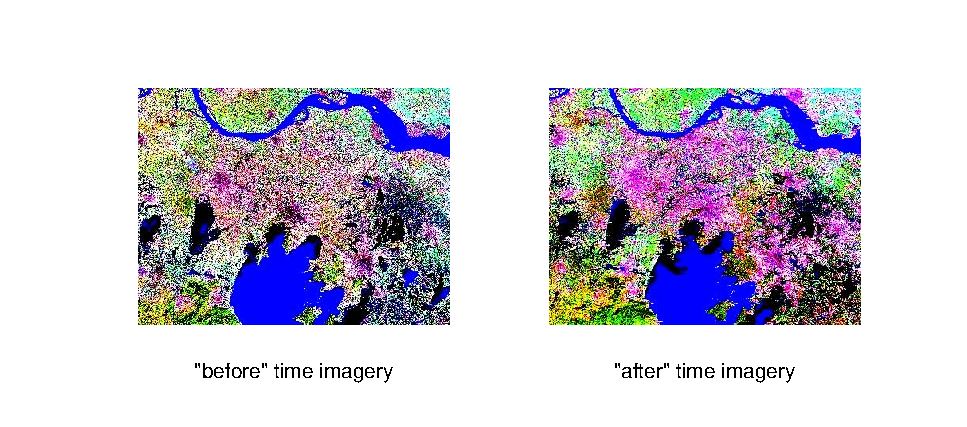
\includegraphics[width=15cm]{tti.eps}
\caption{The Time-series Imageries.}
\label{method}
\end{center}
\end{figure}

Through the investigation of land-cover, we label the five different land-cover types on the pair of time-series RS imageries manually.  
To get the training and testing data sets, five $20\times20$ labeled squares with different land-cover types are labeled on both the "before" and "after" time imageries as shown in firgure 3.
\begin{figure}[tbh]
\begin{center}
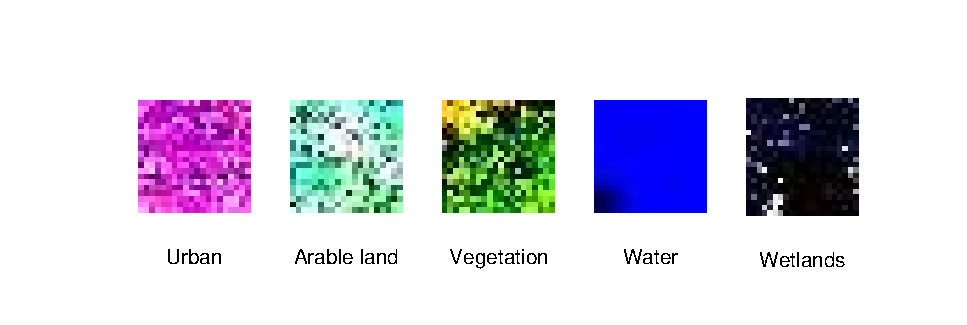
\includegraphics[width=15cm]{samples.eps}
\caption{Five labeled different land-cover samples with the size of $20\times20$ pixels.}
\label{method}
\end{center}
\end{figure}

In this experiment, we collect a training samples set $\chi$ as well as a testing samples set $\psi$ with the size of 3000.
And every sample is a four elements tuple, in which the first three elements are the RGB values of every pixel, while the last element is the label of the pixel. 
\par

We incrementally train and test the ELM network with the hidden node number ranging from 10 to 400 and and an increasing step of 3. 
Moreover, every network are trained and tested 3 times and the average testing accuracy are calculated to assure the accuracy.
The finall result can be represented by figure 4, which shows the networks' testing accuracy trend with different hidden node number and activative function.
From the figure we can firstly conclude that all the activate functions, except for hardlim, performs similarly the the hidden node number increasing.
Secondly, the average testing accuracy of the networks with the activative functions of sig, sin, tribas and hardlim, improves greatly before the hidden node number reaches 100, but are stabilized when the hidden node number reaches about 150.
Finally, we can see that choosing tribas as the activative function and 350 to 400 hidden node number will bring a little better testing accuracy, which is about 0.98, if the application can accept the increase of training time.  
\begin{figure}[tbh]
\begin{center}
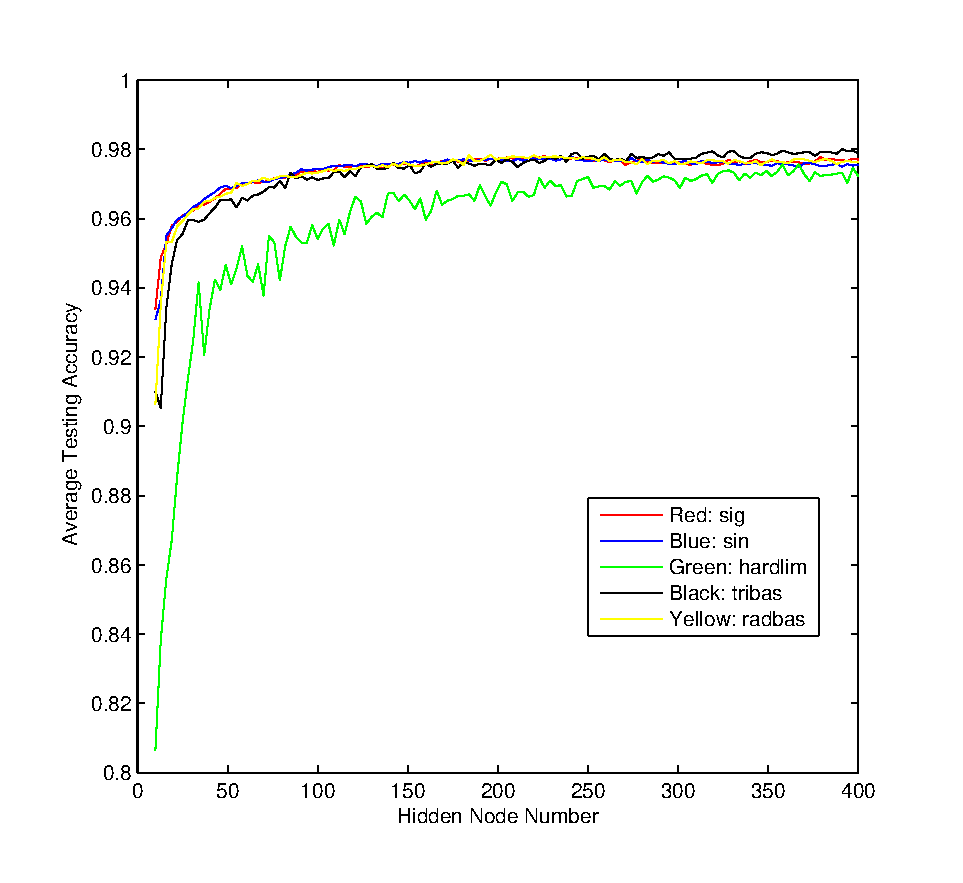
\includegraphics[width=15cm]{itr.eps}
\caption{Incremental ELM Training Result.}
\label{method}
\end{center}
\end{figure}
\par

\subsection{Land-cover Classification Performance of ELM}
The most valuable factors of ELM are the high learning spead and generalisation performance, which are also the two advantages that our land-cover change detection method's accuracy and scability are based on.
In this experiment, we compare ELM to BP and SVM in the application of RS imagery classification. 
\par

One factor that we will compare is their training time, with their generalisation performance ensured.
In this experiment, we set the hidden node number to 100 and use the active function of sin, which can generate an ELM network with testing accuracy of about 0.97 using 3000 training samples and 3000 testing samples.
Similarly, we adjust both the parameters of SVM and BP networks to assure their testing accuracy ranging between 0.95 and 0.96 using the same training and testing samples.
Moreover, we compare the training time of all the methods using increasing training data size, and to specific size of training data, multi training is performed and the average training time is calculated.
The training time comparision result can be seen in figure 5.
\begin{figure}[tbh]
\begin{center}
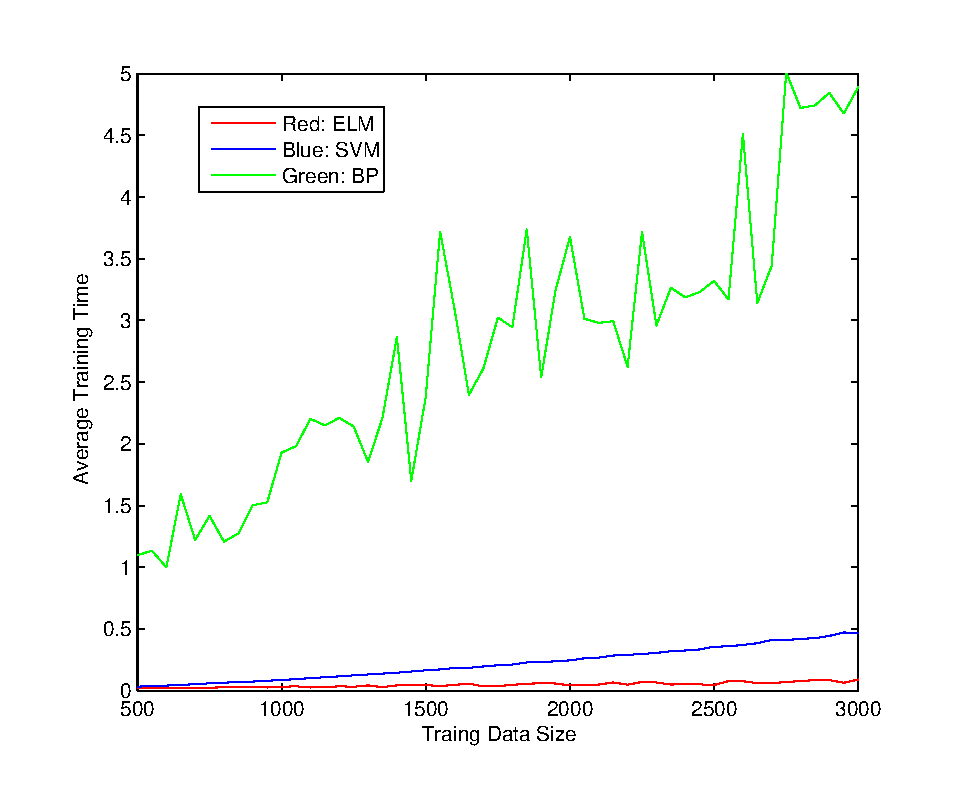
\includegraphics[width=15cm]{tt.eps}
\caption{Average Training Time Comparision. }
\label{method}
\end{center}
\end{figure}
\par

From the figure we can argue that ELM always costs the least training time.
With the increasing training data size, the training time of BP network increases greatly and are unstable.
From the data of figure 6, we can see the BP network takes about 47 times more time than ELM to learn. 
Although SVM network training is much faster than BP network, it still takes nearly 7 times more time to learn than ELM.
\par

\begin{table}[h]
\scriptsize{
\begin{center}
\begin{tabular}[bt]{|c||c|c|c||c|c|c||c|c|c|}\hline

 & \multicolumn{3}{|c||}{ELM} & \multicolumn{3}{|c||}{BP} & \multicolumn{3}{|c|}{SVM} \\ \hline
Size &TrainTime &TestTime &TestAcc &TrainTime &TestTime &TestAcc &TrainTime &TestTime &TestAcc \\ \hline
500 &0.018000 &0.006000 &0.973200 &0.031253 &0.005436 &0.934000 &1.474384 &0.008222 &0.958000 \\ \hline
750 &0.027000 &0.006000 &0.971333 &0.058225 &0.010785 &0.936000 &1.377492 &0.008237 &0.927333 \\ \hline
1000 &0.032000 &0.007000 &0.971000 &0.084406 &0.016624 &0.943000 &1.788723 &0.008306 &0.933300 \\ \hline
1250 &0.037000 &0.006000 &0.971360 &0.117043 &0.023910 &0.945600 &1.755750 &0.008938 &0.957760 \\ \hline
1500 &0.048000 &0.012000 &0.971733 &0.159608 &0.034197 &0.951333 &1.963340 &0.008352 &0.963467 \\ \hline
1750 &0.056000 &0.011000 &0.971429 &0.217431 &0.041878 &0.951429 &2.205566 &0.008535 &0.957943 \\ \hline
2000 &0.061000 &0.012000 &0.974150 &0.247115 &0.051873 &0.955000 &2.311722 &0.008987 &0.939900 \\ \hline
2250 &0.059000 &0.014000 &0.973422 &0.322188 &0.062474 &0.951111 &2.111166 &0.009078 &0.964089 \\ \hline
2500 &0.078000 &0.014000 &0.975560 &0.360570 &0.074148 &0.953200 &2.840775 &0.008804 &0.965120 \\ \hline
2750 &0.080000 &0.015000 &0.975382 &0.416586 &0.087604 &0.952000 &3.348820 &0.009248 &0.959673 \\ \hline
3000 &0.084000 &0.015000 &0.974500 &0.455141 &0.098914 &0.952333 &3.323896 &0.009408 &0.961267 \\ \hline
\end{tabular}
\caption{RS Imagery Classification Performance Comparision among ELM, BP and SVM}
\label{specification}
\end{center}
}
\end{table}

The other factor that we will compare is their testing accuracy, with increasing training and testing samples.

\subsection{Change Detection Result}

\subsection{Scalability}






%%%%%%%%%%%%%%%%%%%%%%%%%%%%%%%%%%%%%%%%%%%%%%%%%%%%%%%%%%%
%%%%%%%%%%%%%        Conclusions      %%%%%%%%%%%%%%%%%%%%%
%%%%%%%%%%%%%%%%%%%%%%%%%%%%%%%%%%%%%%%%%%%%%%%%%%%%%%%%%%%
\section{Conclusions}\label{conclusion}

This paper studies ELM for classification with the standard optimization method. 


\bibliography{/home/jychen/Documents/MachineLearning/mypaper/paper/reference}

\end{document} 
